\section{Mô tả thiết kế phần mềm}
\subsection{Sơ đồ UML của phần mềm}
Do kích thước chiều ngang của giấy có hạn nên sơ đồ UML của phần mềm được đặt trong thư mục \textbf{UMLDiagram}, đính kèm với bản báo cáo này.

\subsection{Mô tả các lớp trong phần mềm}
\subsubsection{Namespace \lstinline{utilities}}
Namespace \lstinline{utilities} cung cấp các hàm bổ trợ cho quá trình xử lý, ví dụ như hàm cung cấp địa chỉ (location) của các hình ảnh, âm thanh, hay hàm kiểm tra vị trí hợp lệ...

\subsubsection{Lớp \lstinline{Settings}}
Lớp \lstinline{Settings} cung cấp một vài thông tin cài dặt cơ bản của game.\\
Sơ đồ UML của lớp \lstinline{Settings} như sau:

\begin{figure}[H]
\centering{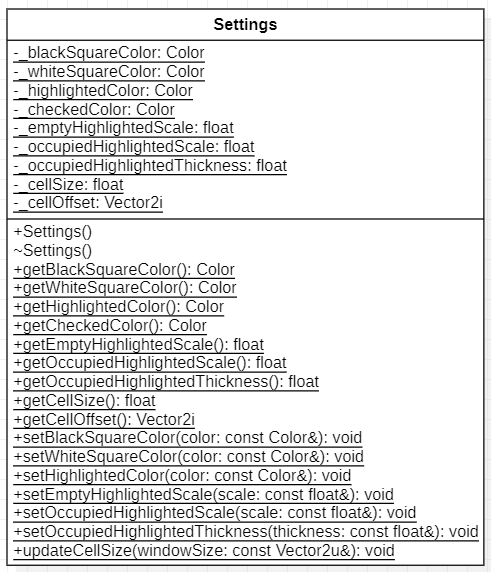
\includegraphics[scale=0.8]{images/classes/Settings}}
\caption{Sơ đồ UML của lớp \lstinline{Settings}}
\end{figure} 

Các thuộc tính (attributes) của lớp \lstinline{Settings} là thông tin về màu của các ô vuông trên bàn cờ, màu của ô vuông lúc được làm nổi bật (highlight), màu của ô vuông khi bị chiếu. Các màu này được dựa trên mã màu RGBA. Mã màu RGGA trong đồ án được lấy từ trang web: \url{https://rgbacolorpicker.com}. Ngoài ra, còn có các thuộc tính mô tả về tỉ lệ, độ dày mỏng của các nét highlight, cũng như kích thước và offset của ô vuông trên bàn cờ.\\
Các phương thức (methods) của lớp \lstinline{Settings} cung cấp các hàm getters và setters cho các thuộc tính của lớp.\\
Hầu hết các thuộc tính và phương thức của lớp \lstinline{Settings} (trừ hàm tạo $-$ constructor và hàm hủy $-$ destructor) đều được khai báo dưới dạng thuộc tính/phương thức tĩnh (\lstinline{method}), tạo ra sự tiện lợi khi ta cần gọi chúng, giúp ta không phải tạo một đối tượng mới mỗi khi muốn sử dụng đến các tính năng này.

\subsubsection{Các lớp enum}
\paragraph{Lớp enum \lstinline{GameSound}}
Lớp \lstinline{GameSound} cung cấp các loại âm thanh của game: âm thanh khi di chuyển quân cờ (MOVE), khi bắt quân (CAPTURE), khi chiếu (CHECK), khi chiếu hết (CHECKMATE) hay khi stalemate (trạng thái mà cả hai bên đều không còn nước nào có thể đi được).\\
Sơ đồ UML của lớp enum \lstinline{GameSound} như sau:
\begin{figure}[H]
\centering{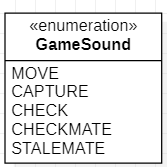
\includegraphics[scale=0.8]{images/classes/GameSound}}
\caption{Sơ đồ UML của lớp enum \lstinline{GameSound}}
\end{figure}

\paragraph{Lớp enum \lstinline{CellStatus}}
Lớp \lstinline{CellStatus} cung cấp các trạng thái của một ô vuông trên bàn cờ: đã có quân (OCCUPIED), chưa có quân (EMPTY) hay đang được highlight (HIGHLIGHTED).\\
Sơ đồ UML của lớp enum \lstinline{CellStatus} như sau:
\begin{figure}[H]
\centering{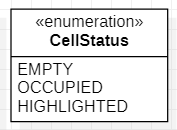
\includegraphics[scale=0.8]{images/classes/CellStatus}}
\caption{Sơ đồ UML của lớp enum \lstinline{CellStatus}}
\end{figure}

\paragraph{Lớp enum \lstinline{MoveType}}
Lớp \lstinline{MoveType} cung cấp thể loại của các nước di chuyển trong game: thăng cấp cho quân Tốt ($\mathrm{PROMOTION}$), nhập thành ngắn ($\mathrm{SHORT\_CASTLING}$), nhập thành dài ($\mathrm{LONG\_CASTLING}$), hoặc không phải các nước đi trên ($\mathrm{NONE}$).\\
Sơ đồ UML của lớp enum \lstinline{MoveType} như sau:
\begin{figure}[H]
\centering{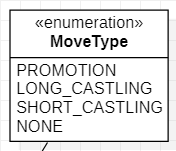
\includegraphics[scale=0.8]{images/classes/MoveType}}
\caption{Sơ đồ UML của lớp enum \lstinline{MoveType}}
\end{figure}

\paragraph{Lớp enum \lstinline{PieceType}}
Lớp \lstinline{PieceType} cung cấp các loại quân cờ: quân Vua (KING), quân Hậu (QUEEN), quân Tượng (BISHOP), quân Mã (KNIGHT), quân Xe (ROOK) và quân Tốt (PAWN).\\
Sơ đồ UML của lớp enum \lstinline{PieceType} như sau:
\begin{figure}[H]
\centering{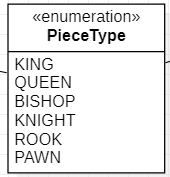
\includegraphics[scale=0.8]{images/classes/PieceType}}
\caption{Sơ đồ UML của lớp enum \lstinline{PieceType}}
\end{figure}

\paragraph{Lớp enum \lstinline{PieceDirection}}
Lớp \lstinline{PieceDirection} cung cấp hướng di chuyển thẳng về phía trước cho quân Tốt: đi lên (UP) đối với Tốt trắng và đi xuống (DOWN) đối với Tốt đen.\\
Sơ đồ UML của lớp enum \lstinline{PieceDirection} như sau:
\begin{figure}[H]
\centering{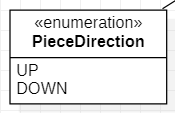
\includegraphics[scale=0.8]{images/classes/PieceDirection}}
\caption{Sơ đồ UML của lớp enum \lstinline{PieceDirection}}
\end{figure}

\paragraph{Lớp enum \lstinline{PieceColor}}
Lớp \lstinline{PieceColor} cho biết hai màu của người chơi/quân cờ: màu trắng (WHITE) và màu đen (BLACK).\\
Sơ đồ UML của lớp enum \lstinline{PieceColor} như sau:
\begin{figure}[H]
\centering{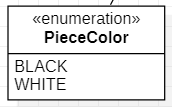
\includegraphics[scale=0.8]{images/classes/PieceColor}}
\caption{Sơ đồ UML của lớp enum \lstinline{PieceColor}}
\end{figure}

\subsubsection{Lớp \lstinline{ChessMove}}
Lớp \lstinline{ChessMove} cung cấp thông tin về nước đi trên bàn cờ.\\
Sơ đồ UML của lớp \lstinline{ChessMove} như sau:
\begin{figure}[H]
\centering{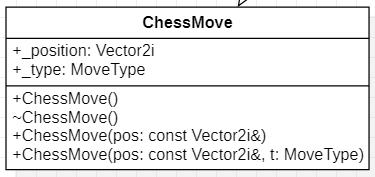
\includegraphics[scale=0.8]{images/classes/ChessMove}}
\caption{Sơ đồ UML của lớp \lstinline{ChessMove}}
\end{figure}
Các thuộc tính của lớp \lstinline{ChessMove} cho biết vị trí và thể loại của nước đi đó.\\
Các phương thức khởi tạo của lớp \lstinline{ChessMove} cho phép ta khởi tạo mặc định, khởi tạo với một tham số và khởi tạo với đầy đủ tham số.

\subsubsection{Lớp \lstinline{Cell}}
Lớp \lstinline{Cell} thể hiện mỗi một ô vuông trên bàn cờ vua.\\
Sơ đồ UML của lớp \lstinline{Cell} như sau:
\begin{figure}[H]
\centering{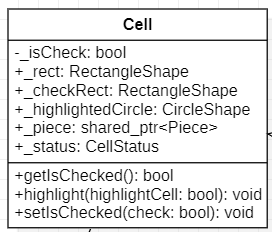
\includegraphics[scale=0.8]{images/classes/Cell}}
\caption{Sơ đồ UML của lớp \lstinline{Cell}}
\end{figure}
Các thuộc tính chính của lớp \lstinline{Cell} gồm có thuộc tính để đánh dấu xem ô này có đang bị chiếu hay không, một con trỏ \lstinline{shared_ptr} trỏ đến một đối tượng thuộc lớp \lstinline{Piece} (sẽ được trình bày trong phần sau) $-$ quân cờ hiện tại ở ô này (nếu ô này đang không bị chiếm giữ bởi quân cờ nào  thì trỏ đến \lstinline{nullptr}), hay thuộc tính thể hiện trạng thái hiện tại của ô vuông này. Ngoài ra, các đối tượng từ lớp \lstinline{RectangleShape} và \lstinline{CircleShape} của thư viện SFML cũng được sử dụng để tạo các thuộc tính nhằm phục vụ cho việc thiết kế giao diện người dùng (GUI).\\
Thuộc tính \lstinline{_piece} có kiểu con trỏ \lstinline{shared_ptr} của thư viện STL để hạn chế tình trạng rò rỉ bộ nhớ (memory leak).

\subsubsection{Lớp \lstinline{Piece}}
Lớp \lstinline{Piece} là một lớp trừu tượng, để biểu diễn một quân cờ tổng quát trên bàn cờ vua.\\
Sơ đồ UML của lớp \lstinline{Piece} như sau:
\begin{figure}[H]
\centering{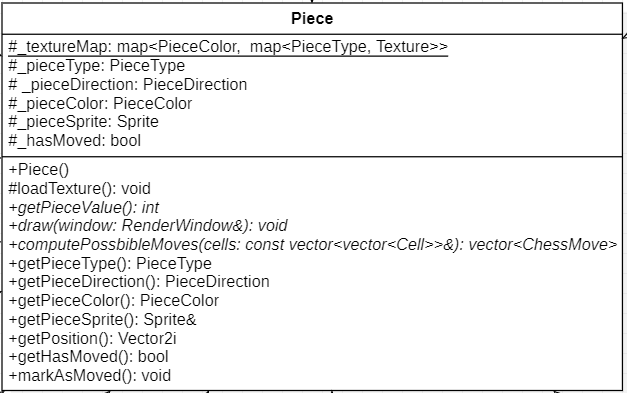
\includegraphics[scale=0.8]{images/classes/Piece}}
\caption{Sơ đồ UML của lớp \lstinline{Piece}}
\end{figure}
Các thuộc tính của lớp \lstinline{Piece} được khai báo \lstinline{protected} để cho các lớp kế thừa từ nó có thể truy cập vào các thuộc tính.\\
Lớp \lstinline{Piece} có thuộc tính tĩnh \lstinline{_textureMap} lưu trữ các \lstinline{Texture} của lần lượt từng quân cờ của mỗi màu. Lớp \lstinline{Texture} và \lstinline{Sprite} được sử dụng từ thư viện SFML.\\
Các thuộc tính khác thể hiện màu sắc, loại quân cờ, hướng di chuyển cùng với một thuộc tính để kiểm tra xem quân cờ này đã di chuyển hay chưa.\\
Lớp này cung cấp các getters, setters cho các thuộc tính, phương thức dùng để tải (load) các Texture. Ngoài ra, lớp \lstinline{Piece} còn cung cấp các phương thức thuần ảo nhằm tận dụng tính đa hình (polymorphism). Các phương thức thuần ảo này sẽ được cài đặt trong các lớp kế thừa cho phù hợp.\\
Trong các lớp kế thừa từ lớp \lstinline{Piece} (6 lớp được trình bày tiếp theo), các thuật toán tìm nước đi khả dĩ (possible moves) của quân cờ được lấy từ: \url{https://github.com/mbusy/chess/tree/master/src}.

\subsubsection{Lớp \lstinline{King}}
Lớp \lstinline{King} là một lớp con kế thừa từ lớp \lstinline{Piece}, thể hiện quân Vua trên bàn cờ. Do là một lớp kế thừa nên nó kế thừa lại tất cả các thuộc tính và phương thức của lớp \lstinline{Piece}. Các phương thức thuần ảo của lớp \lstinline{Piece} được viết lại trong lớp \lstinline{King}.\\
Sơ đồ UML của lớp \lstinline{King} như sau:
\begin{figure}[H]
\centering{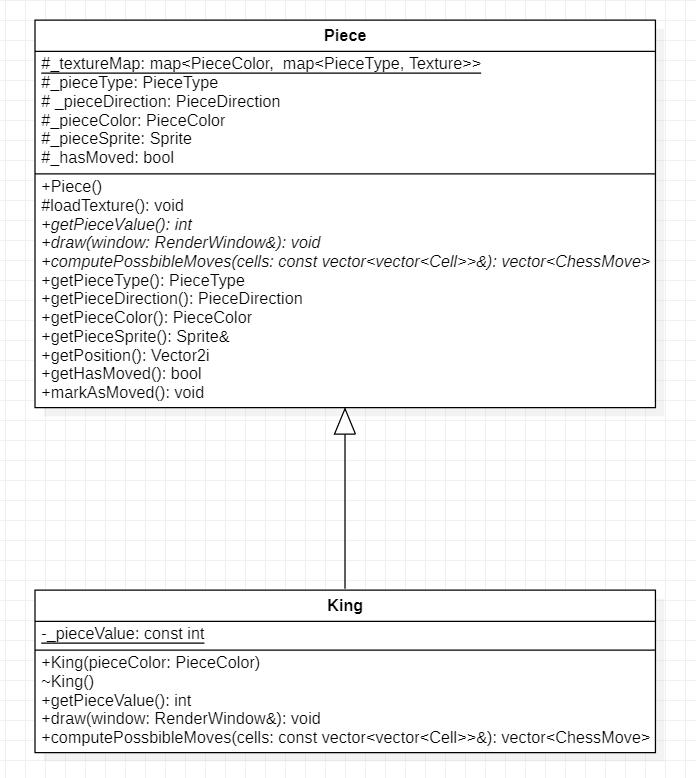
\includegraphics[scale=0.6]{images/classes/King}}
\caption{Sơ đồ UML của lớp \lstinline{King}}
\end{figure}
Hình sau mô tả các nước đi có thể của quân Vua, được viết trong phương thức \lstinline{computePossibleMoves}.
\begin{figure}[H]
\centering{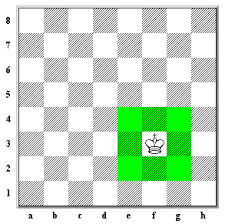
\includegraphics[scale=0.6]{images/moves/King}}
\caption{Các nước đi của quân Vua. Nguồn: \url{chesscorner.com}}
\end{figure}

\subsubsection{Lớp \lstinline{Queen}}
Lớp \lstinline{Queen} là một lớp con kế thừa từ lớp \lstinline{Piece}, thể hiện quân Hậu trên bàn cờ. Do là một lớp kế thừa nên nó kế thừa lại tất cả các thuộc tính và phương thức của lớp \lstinline{Piece}. Các phương thức thuần ảo của lớp \lstinline{Piece} được viết lại trong lớp \lstinline{Queen}.\\
Sơ đồ UML của lớp \lstinline{Queen} như sau:
\begin{figure}[H]
\centering{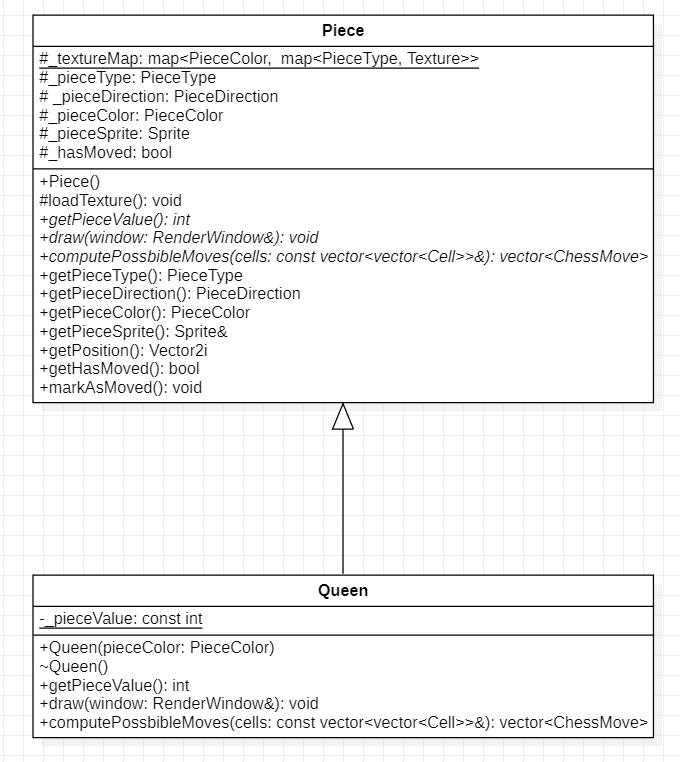
\includegraphics[scale=0.6]{images/classes/Queen}}
\caption{Sơ đồ UML của lớp \lstinline{Queen}}
\end{figure}
Hình sau mô tả các nước đi có thể của quân Hậu, được viết trong phương thức \lstinline{computePossibleMoves}.
\begin{figure}[H]
\centering{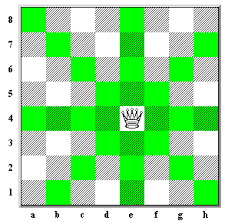
\includegraphics[scale=0.6]{images/moves/Queen}}
\caption{Các nước đi của quân Hậu. Nguồn: \url{chesscorner.com}}
\end{figure}

\subsubsection{Lớp \lstinline{Bishop}}
Lớp \lstinline{Bishop} là một lớp con kế thừa từ lớp \lstinline{Piece}, thể hiện quân Tượng trên bàn cờ. Do là một lớp kế thừa nên nó kế thừa lại tất cả các thuộc tính và phương thức của lớp \lstinline{Piece}. Các phương thức thuần ảo của lớp \lstinline{Piece} được viết lại trong lớp \lstinline{Bishop}.\\
Sơ đồ UML của lớp \lstinline{Bishop} như sau:
\begin{figure}[H]
\centering{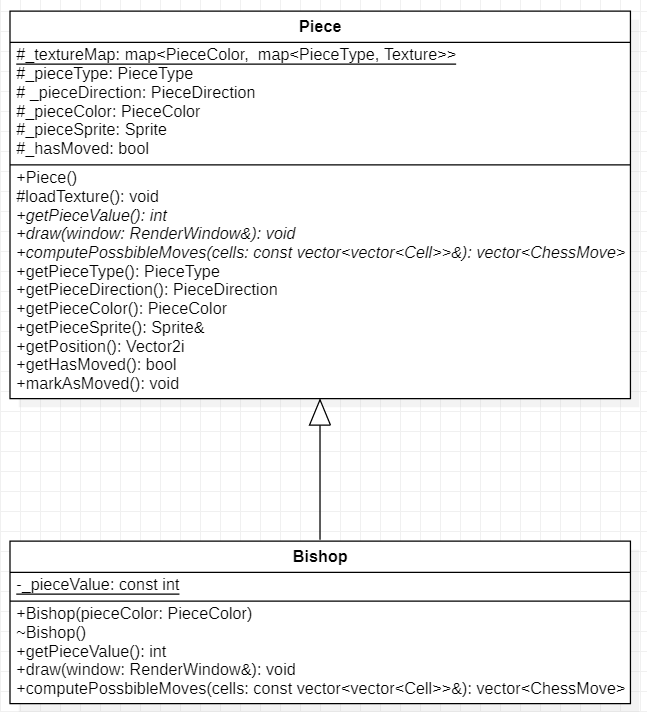
\includegraphics[scale=0.6]{images/classes/Bishop}}
\caption{Sơ đồ UML của lớp \lstinline{Bishop}}
\end{figure}
Hình sau mô tả các nước đi có thể của quân Tượng, được viết trong phương thức \lstinline{computePossibleMoves}.
\begin{figure}[H]
\centering{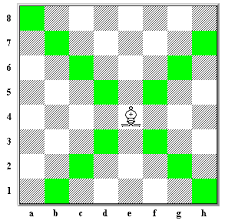
\includegraphics[scale=0.6]{images/moves/Bishop}}
\caption{Các nước đi của quân Tượng. Nguồn: \url{chesscorner.com}}
\end{figure}

\subsubsection{Lớp \lstinline{Knight}}
Lớp \lstinline{Knight} là một lớp con kế thừa từ lớp \lstinline{Piece}, thể hiện quân Mã trên bàn cờ. Do là một lớp kế thừa nên nó kế thừa lại tất cả các thuộc tính và phương thức của lớp \lstinline{Piece}. Các phương thức thuần ảo của lớp \lstinline{Piece} được viết lại trong lớp \lstinline{Knight}.\\
Sơ đồ UML của lớp \lstinline{Knight} như sau:
\begin{figure}[H]
\centering{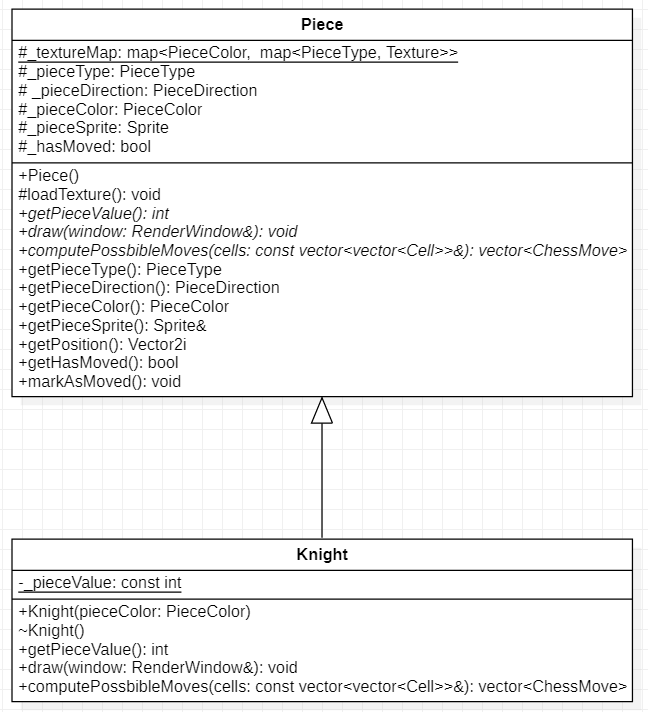
\includegraphics[scale=0.6]{images/classes/Knight}}
\caption{Sơ đồ UML của lớp \lstinline{Knight}}
\end{figure}
Hình sau (các ô màu đỏ) mô tả các nước đi có thể của quân Mã, được viết trong phương thức \lstinline{computePossibleMoves}.
\begin{figure}[H]
\centering{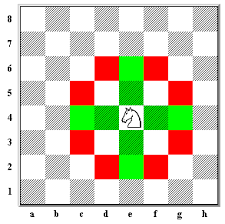
\includegraphics[scale=0.6]{images/moves/Knight}}
\caption{Các nước đi của quân Mã. Nguồn: \url{chesscorner.com}}
\end{figure}

\subsubsection{Lớp \lstinline{Rook}}
Lớp \lstinline{Rook} là một lớp con kế thừa từ lớp \lstinline{Piece}, thể hiện quân Xe trên bàn cờ. Do là một lớp kế thừa nên nó kế thừa lại tất cả các thuộc tính và phương thức của lớp \lstinline{Piece}. Các phương thức thuần ảo của lớp \lstinline{Piece} được viết lại trong lớp \lstinline{Rook}.\\
Sơ đồ UML của lớp \lstinline{Rook} như sau:
\begin{figure}[H]
\centering{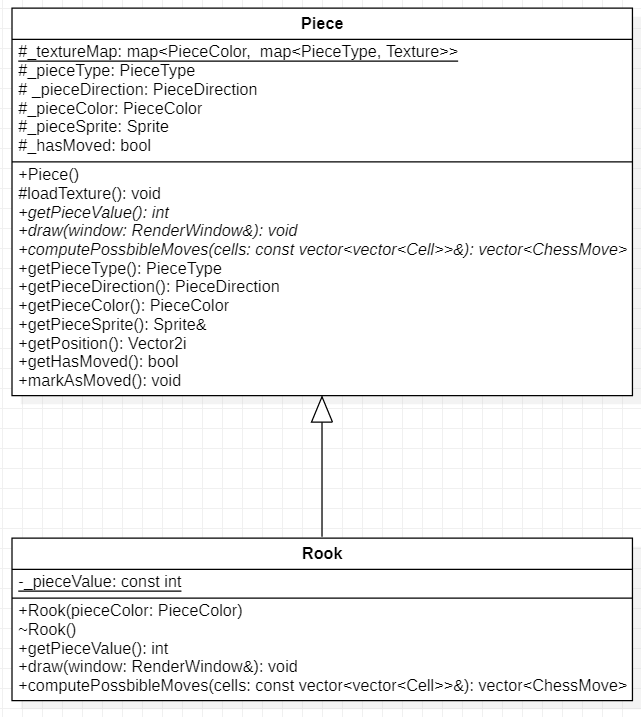
\includegraphics[scale=0.6]{images/classes/Rook}}
\caption{Sơ đồ UML của lớp \lstinline{Rook}}
\end{figure}
Hình sau mô tả các nước đi có thể của quân Xe, được viết trong phương thức \lstinline{computePossibleMoves}.
\begin{figure}[H]
\centering{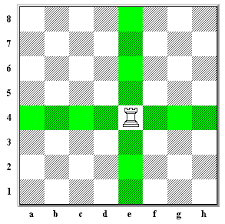
\includegraphics[scale=0.6]{images/moves/Rook}}
\caption{Các nước đi của quân Xe. Nguồn: \url{chesscorner.com}}
\end{figure}

\subsubsection{Lớp \lstinline{Pawn}}
Lớp \lstinline{Pawn} là một lớp con kế thừa từ lớp \lstinline{Piece}, thể hiện quân Tốt trên bàn cờ. Do là một lớp kế thừa nên nó kế thừa lại tất cả các thuộc tính và phương thức của lớp \lstinline{Piece}. Các phương thức thuần ảo của lớp \lstinline{Piece} được viết lại trong lớp \lstinline{Pawn}.\\
Sơ đồ UML của lớp \lstinline{Pawn} như sau:
\begin{figure}[H]
\centering{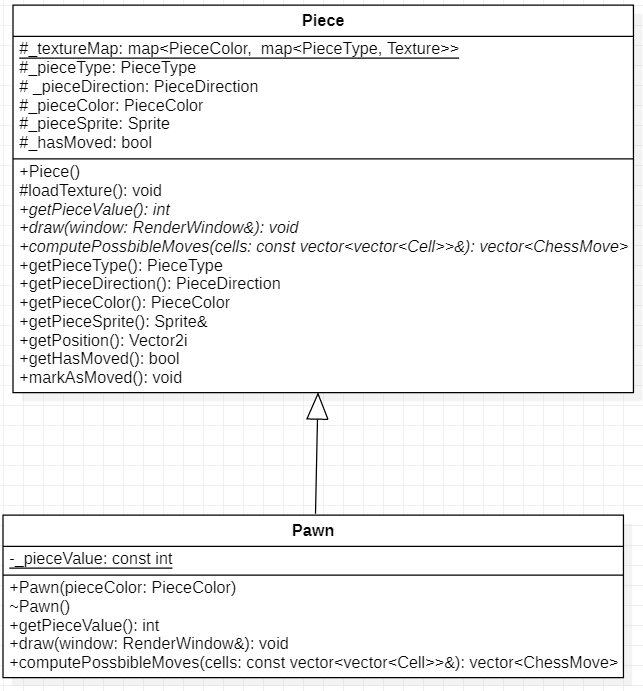
\includegraphics[scale=0.6]{images/classes/Pawn}}
\caption{Sơ đồ UML của lớp \lstinline{Pawn}}
\end{figure}
Hình sau mô tả các nước đi có thể của quân Tốt, được viết trong phương thức \lstinline{computePossibleMoves}.
\begin{figure}[H]
\centering{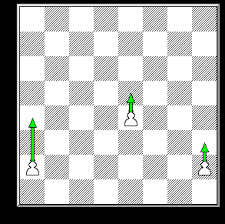
\includegraphics[scale=0.6]{images/moves/Pawn}}
\caption{Các nước đi của quân Tốt. Nguồn: \url{chesscorner.com}}
\end{figure}
Việc phong cấp cho quân Tốt sẽ được xử lý ở lớp \lstinline{ChessBoard}, được trình bày ở phần sau.

\subsubsection{Lớp \lstinline{AudioPlayer}}
Lớp \lstinline{AudioPlayer} chủ yếu cung cấp cho ta các phương thức liên quan đến việc xử lý âm thanh của game (load, play, pause, resume, stop).\\
Sơ đồ UML của lớp \lstinline{AudioPlayer} như sau:
\begin{figure}[H]
\centering{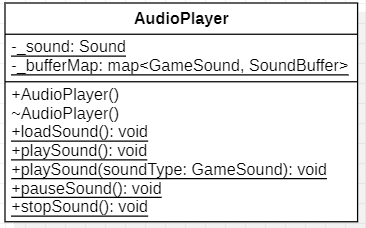
\includegraphics[scale=0.6]{images/classes/AudioPlayer}}
\caption{Sơ đồ UML của lớp \lstinline{AudioPlayer}}
\end{figure}

\subsubsection{Lớp \lstinline{GameUser}}
Lớp \lstinline{GameUser} thể hiện người dùng game Cờ vua (bên trắng và bên đen).\\
Sơ đồ UML của lớp \lstinline{GameUser} như sau:
\begin{figure}[H]
\centering{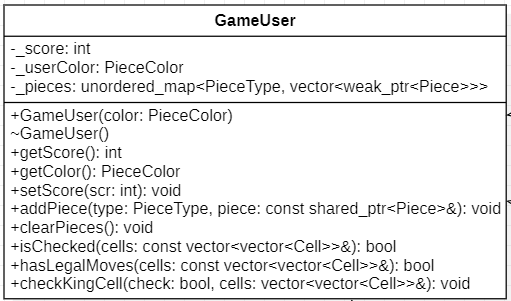
\includegraphics[scale=0.6]{images/classes/GameUser}}
\caption{Sơ đồ UML của lớp \lstinline{GameUser}}
\end{figure}
Các thuộc tính của lớp \lstinline{GameUser} gồm có điểm, màu, và các quân cờ. Con trỏ \lstinline{weak_ptr} của thư viện STL được sử dụng để tham chiếu đến đối tượng được quản lý bởi \lstinline{shared_ptr}.\\
Các thuộc tính của lớp \lstinline{GameUser} bao gồm các getters, setters, các hàm giúp ta thêm các quân cờ, kiểm tra xem người dùng có đang bị chiếu hay không, kiểm tra xem người dùng còn nước đi hợp lệ nào hay không, hay phương thức dùng để chiếu người dùng.

\subsubsection{Lớp \lstinline{ChessBoard}}
Lớp \lstinline{ChessBoard} thể hiện bàn cờ của game Cờ vua trên cửa sổ game.\\
Sơ đồ UML của lớp \lstinline{ChessBoard} như sau:
\begin{figure}[H]
\centering{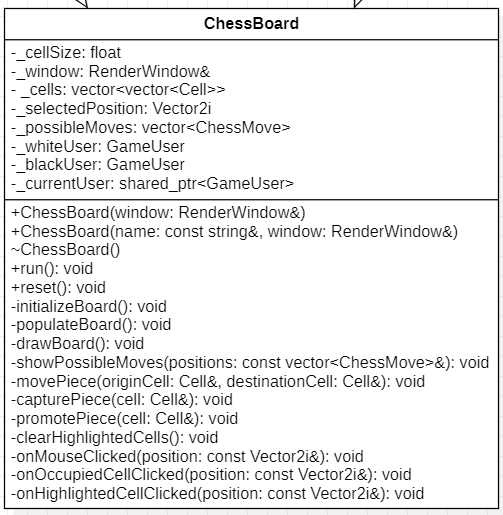
\includegraphics[scale=0.6]{images/classes/ChessBoard}}
\caption{Sơ đồ UML của lớp \lstinline{ChessBoard}}
\end{figure}
Các thuộc tính chủ yếu của lớp \lstinline{ChessBoard} gồm cửa sổ game, mảng hai chiều các ô vuông trên bàn cờ, các nước đi có thể có, người chơi màu trắng, người chơi màu đen và người chơi hiện tại của game.\\
Các phương thức có tầm vực \lstinline{public} của lớp \lstinline{ChessBoard} gồm các phương thức \lstinline{run()}, là phương thức chủ yếu để biểu diễn bàn cờ lên GUI, và phương thức \lstinline{reset()} dùng để reset bàn cờ.\\
Ngoài ra, lớp \lstinline{ChessBoard} còn gồm nhiều phương thức có tầm vực \lstinline{private}:
\begin{itemize}
 \item Phương thức \lstinline{initializeBoard} dùng để khởi tạo một bàn cờ.
 \item Phương thức \lstinline{populateBoard}, dùng để đặt các quân cờ vào vị trí trên bàn cờ.
  \item Phương thức \lstinline{drawBoard}, dùng để hiển thị bàn cờ ra màn hình.
  \item Phương thức \lstinline{showPossibleMoves}, dùng để hiển thị những nước đi khả dĩ của quân cờ được chọn hiện tại.
  \item Phương thức \lstinline{movePiece}, dùng để di chuyển một quân cờ.
  \item Phương thức \lstinline{capturePiece}, dùng để bắt (ăn) một quân cờ khác.
  \item Phương thức \lstinline{promotePiece}, dùng để phong cấp cho quân Tốt khi đạt đủ điều kiện.
  \item Ngoài ra, còn các phương thức xử lý những cú click chuột trên cửa sổ game.
\end{itemize} 